\documentclass[portrait,final,a0paper]{baposter}
%\documentclass[a4shrink,portrait,final]{baposter}
% Usa a4shrink for an a4 sized paper.

\tracingstats=2

\usepackage{calc}
\usepackage{graphicx}
\usepackage{amsmath}
\usepackage{amssymb}
\usepackage{relsize}
\usepackage{multirow}
\usepackage{bm}
\usepackage{graphicx}
\usepackage{multicol}
\usepackage{ marvosym }
\usepackage[utf8]{inputenc}
\DeclareUnicodeCharacter{00A0}{ }
\usepackage{pgfbaselayers}
\pgfdeclarelayer{background}
\pgfdeclarelayer{foreground}
\pgfsetlayers{background,main,foreground}
\usepackage{times}
\usepackage{helvet}
%\usepackage{bookman}
\usepackage{palatino}

\newcommand{\captionfont}{\footnotesize}

\selectcolormodel{cmyk}

\graphicspath{{images/}}

%%%%%%%%%%%%%%%%%%%%%%%%%%%%%%%%%%%%%%%%%%%%%%%%%%%%%%%%%%%%%%%%%%%%%%%%%%%%%%%%
%%%% Some math symbols used in the text
%%%%%%%%%%%%%%%%%%%%%%%%%%%%%%%%%%%%%%%%%%%%%%%%%%%%%%%%%%%%%%%%%%%%%%%%%%%%%%%%
% Format 
\newcommand{\Matrix}[1]{\begin{bmatrix} #1 \end{bmatrix}}
\newcommand{\Vector}[1]{\Matrix{#1}}
\newcommand*{\SET}[1]  {\ensuremath{\mathcal{#1}}}
\newcommand*{\MAT}[1]  {\ensuremath{\mathbf{#1}}}
\newcommand*{\VEC}[1]  {\ensuremath{\bm{#1}}}
\newcommand*{\CONST}[1]{\ensuremath{\mathit{#1}}}
\newcommand*{\norm}[1]{\mathopen\| #1 \mathclose\|}% use instead of $\|x\|$
\newcommand*{\abs}[1]{\mathopen| #1 \mathclose|}% use instead of $\|x\|$
\newcommand*{\absLR}[1]{\left| #1 \right|}% use instead of $\|x\|$

\def\norm#1{\mathopen\| #1 \mathclose\|}% use instead of $\|x\|$
\newcommand{\normLR}[1]{\left\| #1 \right\|}% use instead of $\|x\|$

%%%%%%%%%%%%%%%%%%%%%%%%%%%%%%%%%%%%%%%%%%%%%%%%%%%%%%%%%%%%%%%%%%%%%%%%%%%%%%%%
% Multicol Settings
%%%%%%%%%%%%%%%%%%%%%%%%%%%%%%%%%%%%%%%%%%%%%%%%%%%%%%%%%%%%%%%%%%%%%%%%%%%%%%%%
\setlength{\columnsep}{0.7em}
\setlength{\columnseprule}{0mm}


%%%%%%%%%%%%%%%%%%%%%%%%%%%%%%%%%%%%%%%%%%%%%%%%%%%%%%%%%%%%%%%%%%%%%%%%%%%%%%%%
% Save space in lists. Use this after the opening of the list
%%%%%%%%%%%%%%%%%%%%%%%%%%%%%%%%%%%%%%%%%%%%%%%%%%%%%%%%%%%%%%%%%%%%%%%%%%%%%%%%
\newcommand{\compresslist}{%
\setlength{\itemsep}{1pt}%
\setlength{\parskip}{0pt}%
\setlength{\parsep}{0pt}%
}


%%%%%%%%%%%%%%%%%%%%%%%%%%%%%%%%%%%%%%%%%%%%%%%%%%%%%%%%%%%%%%%%%%%%%%%%%%%%%%
%%% Begin of Document
%%%%%%%%%%%%%%%%%%%%%%%%%%%%%%%%%%%%%%%%%%%%%%%%%%%%%%%%%%%%%%%%%%%%%%%%%%%%%%

\begin{document}

%%%%%%%%%%%%%%%%%%%%%%%%%%%%%%%%%%%%%%%%%%%%%%%%%%%%%%%%%%%%%%%%%%%%%%%%%%%%%%
%%% Here starts the poster
%%%---------------------------------------------------------------------------
%%% Format it to your taste with the options
%%%%%%%%%%%%%%%%%%%%%%%%%%%%%%%%%%%%%%%%%%%%%%%%%%%%%%%%%%%%%%%%%%%%%%%%%%%%%%
% Define some colors
\definecolor{silver}{cmyk}{0,0,0,0.3}
\definecolor{yellow}{cmyk}{0,0,0.9,0.0}
\definecolor{reddishyellow}{cmyk}{0,0.22,1.0,0.0}
\definecolor{black}{cmyk}{0,0,0.0,1.0}
\definecolor{darkYellow}{cmyk}{0,0,1.0,0.5}
\definecolor{darkSilver}{cmyk}{0,0,0,0.1}

\definecolor{lightyellow}{cmyk}{0,0,0.3,0.0}
\definecolor{lighteryellow}{cmyk}{0,0,0.1,0.0}
\definecolor{lighteryellow}{cmyk}{0,0,0.1,0.0}
\definecolor{lightestyellow}{cmyk}{0,0,0.05,0.0}

%%
\typeout{Poster Starts}
\background{
  \begin{tikzpicture}[remember picture,overlay]%
    \draw (current page.north west)+(-2em,2em) node[anchor=north west] {\includegraphics[height=1.1\textheight]{silhouettes_background}};
  \end{tikzpicture}%
}

\newlength{\leftimgwidth}
\begin{poster}%
  % Poster Options
  {
  % Show grid to help with alignment
  grid=false,
  % Column spacing
  colspacing=1em,
  % Color style
  bgColorOne=lighteryellow,
  bgColorTwo=lightestyellow,
  borderColor=reddishyellow,
  headerColorOne=yellow,
  headerColorTwo=reddishyellow,
  headerFontColor=black,
  boxColorOne=lightyellow,
  boxColorTwo=lighteryellow,
  % Format of textbox
  textborder=roundedleft,
%  textborder=rectangle,
  % Format of text header
  eyecatcher=true,
  headerborder=open,
  headerheight=0.08\textheight,
  headershape=roundedright,
  headershade=plain,
  headerfont=\Large\textsf, %Sans Serif
  boxshade=plain,
%  background=shade-tb,
  background=plain,
  linewidth=2pt
  }
  % Eye Catcher
  {
\includegraphics[width=8em]{Giraffe-icon.png}} % No eye catcher for this poster. (eyecatcher=no above). If an eye catcher is present, the title is centered between eye-catcher and logo.
  % Title
  {\sf %Sans Serif
  %\bf% Serif
   Graphical Interface for Automatic Function Embedding}
  % Authors
  {\sf %Sans Serif
  % Serif
  \vspace{0.5em}
  Nicolas Herbaut, David Bourasseau, Daniel Negru
  }
  % University logo
    
    
  

  \tikzstyle{light shaded}=[top color=baposterBGtwo!30!white,bottom color=baposterBGone!30!white,shading=axis,shading angle=30]

  % Width of left inset image
     \setlength{\leftimgwidth}{0.78em+8.0em}

%%%%%%%%%%%%%%%%%%%%%%%%%%%%%%%%%%%%%%%%%%%%%%%%%%%%%%%%%%%%%%%%%%%%%%%%%%%%%%
%%% Now define the boxes that make up the poster
%%%---------------------------------------------------------------------------
%%% Each box has a name and can be placed absolutely or relatively.
%%% The only inconvenience is that you can only specify a relative position 
%%% towards an already declared box. So if you have a box attached to the 
%%% bottom, one to the top and a third one which should be in between, you 
%%% have to specify the top and bottom boxes before you specify the middle 
%%% box.
%%%%%%%%%%%%%%%%%%%%%%%%%%%%%%%%%%%%%%%%%%%%%%%%%%%%%%%%%%%%%%%%%%%%%%%%%%%%%%
    %
    % A coloured circle useful as a bullet with an adjustably strong filling
    \newcommand{\colouredcircle}[1]{%
      \tikz{\useasboundingbox (-0.2em,-0.32em) rectangle(0.2em,0.32em); \draw[draw=black,fill=baposterBGone!80!black!#1!white,line width=0.03em] (0,0) circle(0.18em);}}


  \headerbox{Contribution}{name=contribution,column=0,row=0}{
  \vspace{0.3em}
   
   We are demonstrating an application that allows \textbf{Internet Service Provider} (ISP) to provision \textbf{Virtual Content Delivery Network} (vCDN) on their network topology.
   
   We aim at establishing a possible \textbf{collaboration between ISP and CDN operators} that would allows the latters to embed a vCDN Service in an operator network by specifying a Service Level Agreement (SLA) Constract that would keep ISP topology private while letting the CDN controlling some low level network capabilities of content delivery.
   
   Our algorithm increased the request acceptance rate by 52\% and decreased the consumed bandwidth by 31\%.
   
   
   \vspace{1em}
   \textbf{Keywords}: \textit{Service Function Chaining, Virtual Network Functions, ISP, CDN, Collaboration, Software Defined Networks}


 }
   \headerbox{High Level Architecture}{name=project,column=1,span=2,row=0}{

   \begin{multicols}{2}
	   
			
			\begin{minipage}{0.54\textwidth}
			\vspace{1em}
				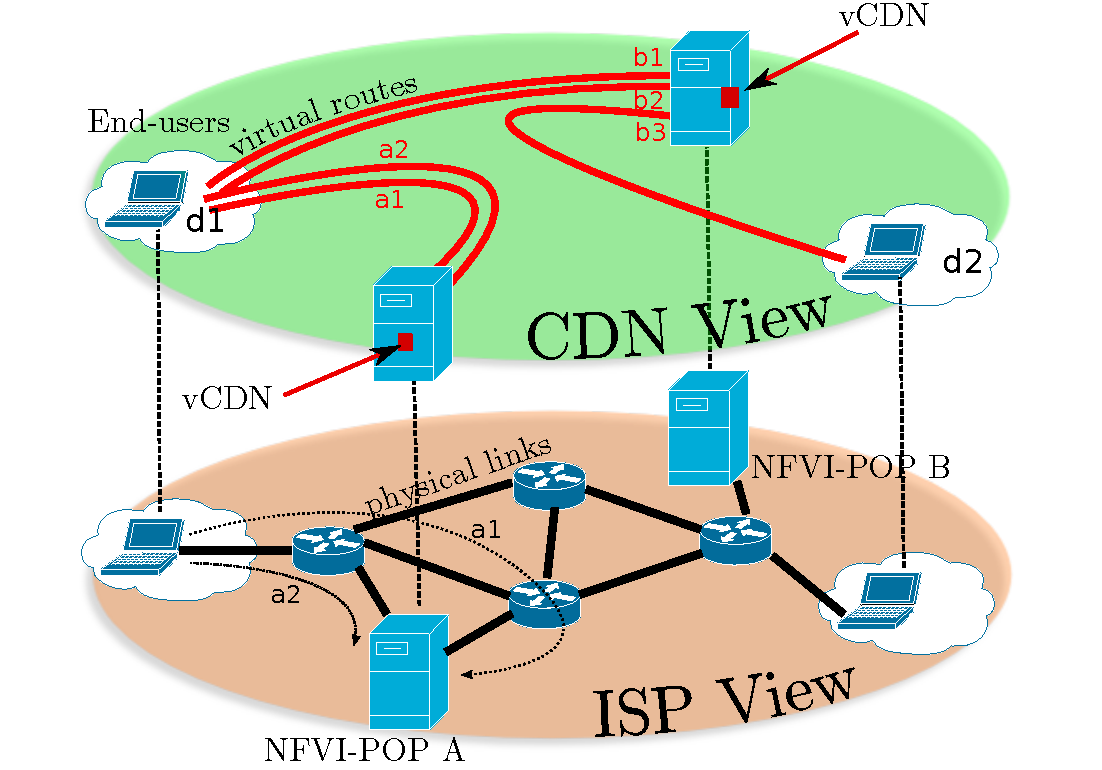
\includegraphics[width=\textwidth]{proposal.pdf}
				\begin{center}\textbf{VCDN deployed in ISP Network}
				
				\end{center}
				
			\end{minipage}
			
				
			\begin{itemize}
				\item Goal: Instantiate a NFV platform within the ISP Network capable of hosting (VCDN) services
				\item ISP manged NFVI-Point of Presence (POPs) are at the edge of the network, interconnected by physical links and switches that support SDN.
				\item CDN manages a "CDN View" overlay that abstracts the ISP Topology
				\item CDN providers manage CDN operations dynamically through an API eg. to decide which route is used, react to route congestion.
			\end{itemize}
			
			
	\end{multicols}
    }
 
   \headerbox{Service Level Agreements}{name=sla,column=0,row=0,below=contribution}{
   
   \begin{itemize}
  \item SLAs are a way to formalize the CDN "demand" for connectivity. ISP responds to the SLA by pricing to the connectivity "offer" they supply. 
  \item On top of video-streaming specific input, SLA contains the User area to be connected as well as the connection to the external CDN network through peering points.
	   
   \end{itemize}
  
  
  \begin{center}
   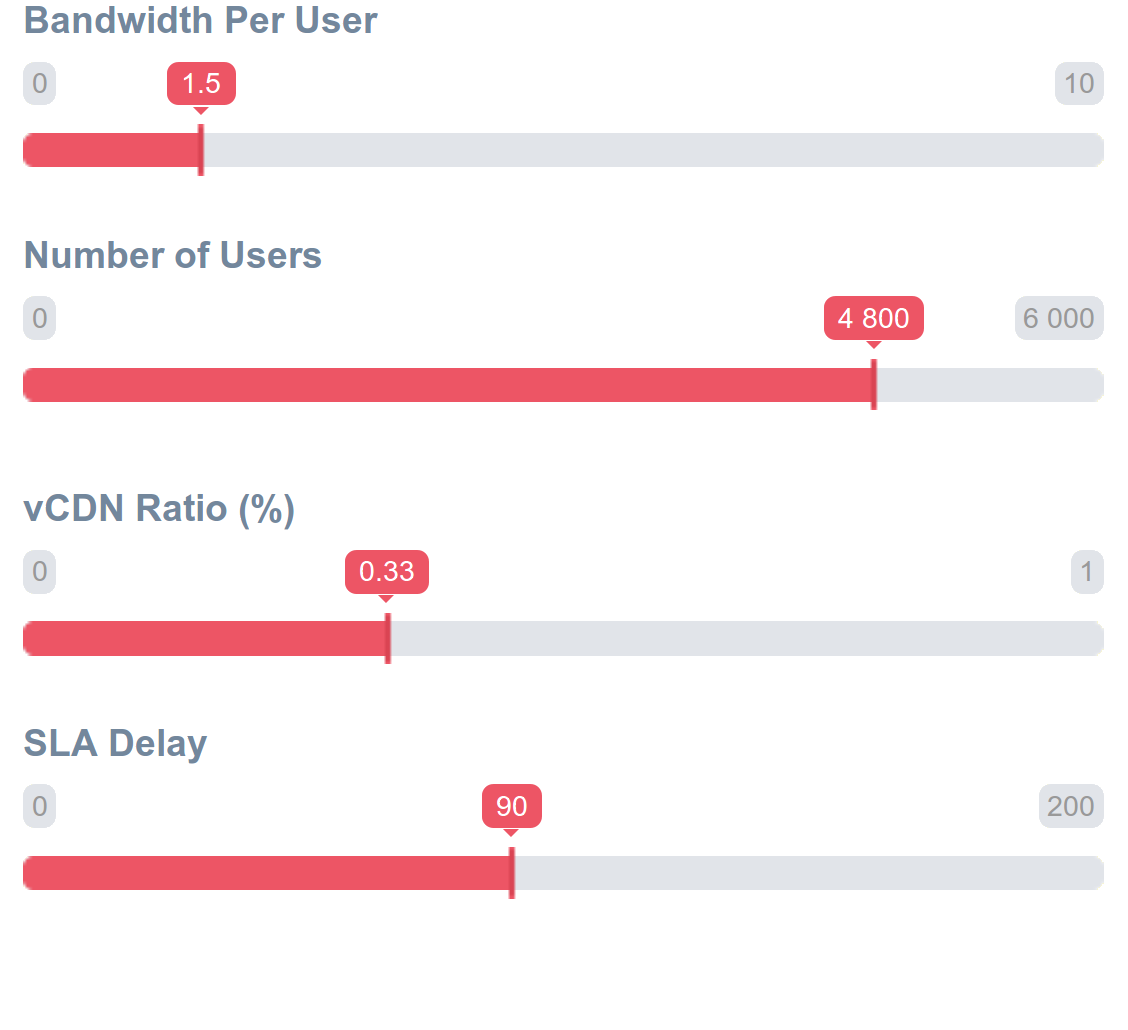
\includegraphics[width=\textwidth]{sla.png}
   \textbf{Sample SLA}
   \end{center}
   
   
   
   
   
	


 }
   \headerbox{Results}{name=results,column=1,span=2,row=0,below=project}{
   
   \begin{multicols}{2}
		   \begin{minipage}{0.6\textwidth}
						\colorbox{white}{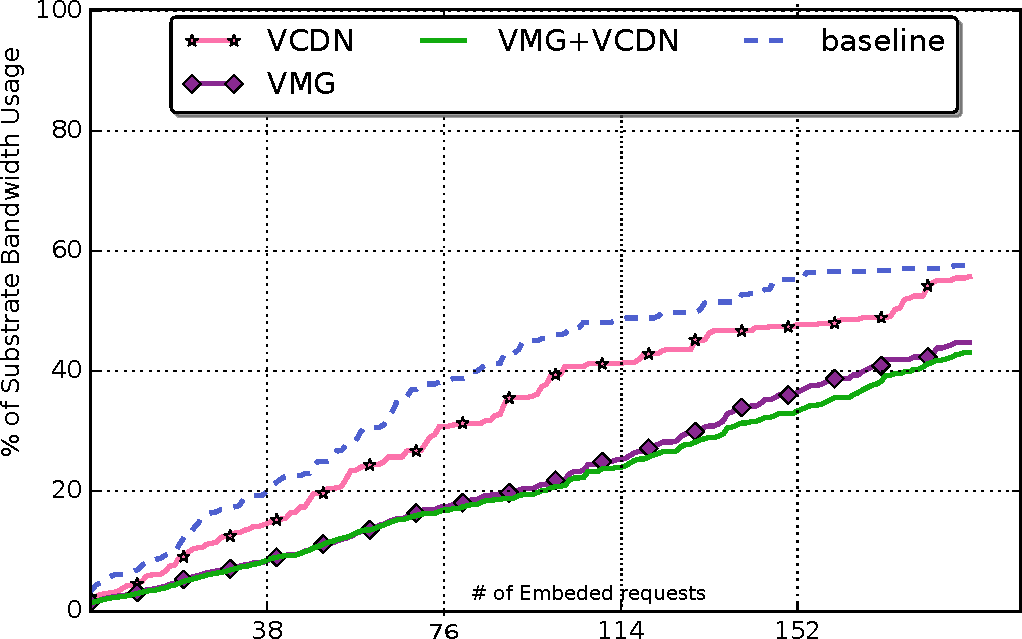
\includegraphics[width=0.8\textwidth]{0-edge-capacities.pdf}}
						\begin{center}\textbf{Edge Capacity}
						\end{center}
					\end{minipage}
				
\begin{minipage}{0.6\textwidth}
\vspace{3em}
						\colorbox{white}{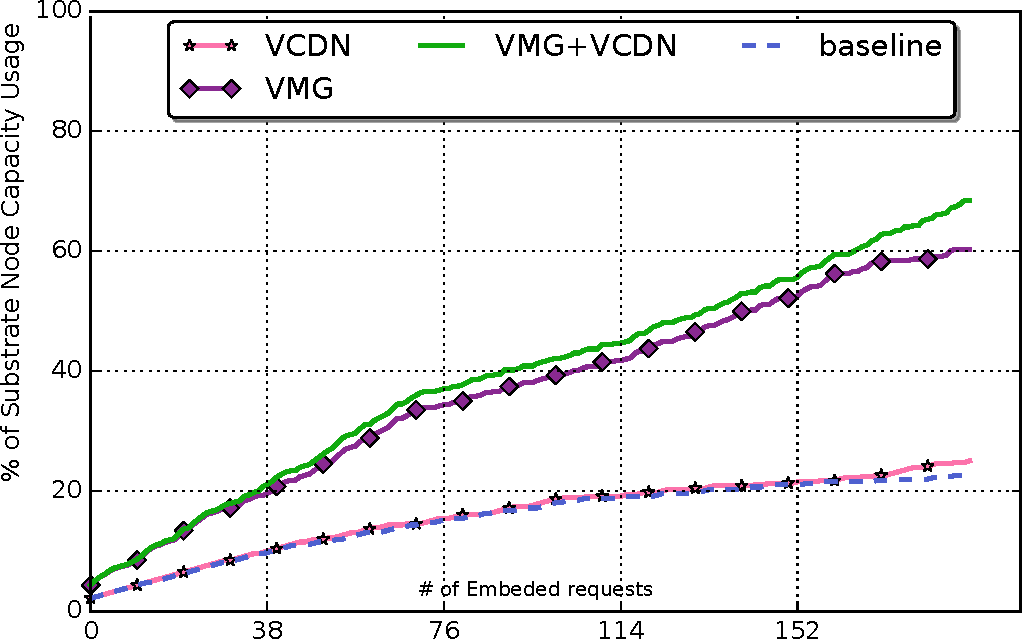
\includegraphics[width=0.8\textwidth]{0-node-capacitie.pdf}}
						\begin{center}\textbf{Node Capacity}
						
						\end{center}
					\end{minipage}
					
\begin{minipage}{0.6\textwidth}
						\colorbox{white}{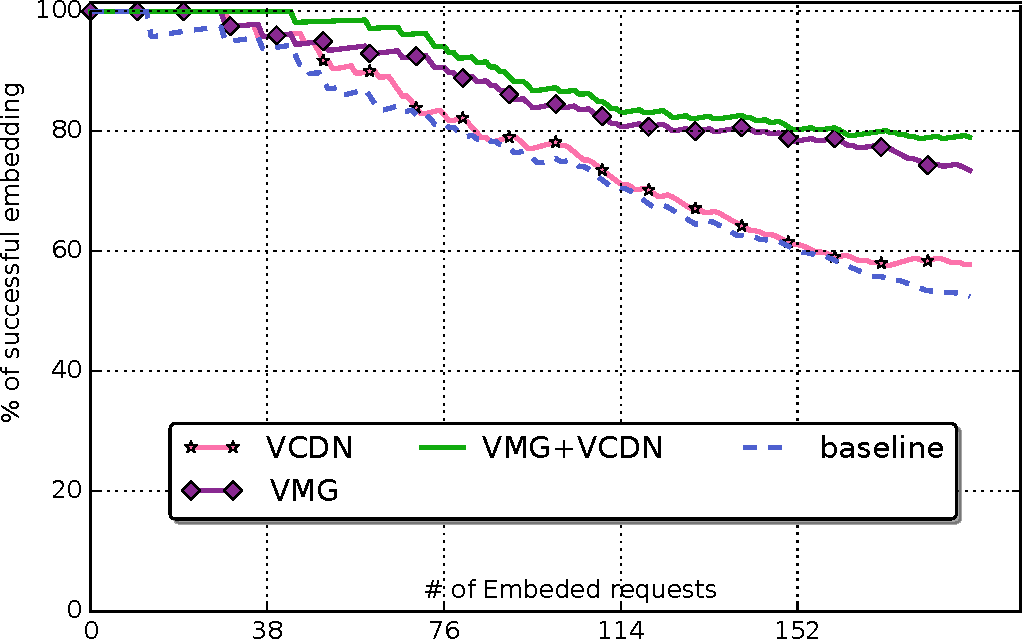
\includegraphics[width=0.8\textwidth]{0-embedding.pdf}}
						\begin{center}\textbf{Embedding Rate}
					
						\end{center}
					\end{minipage}
				
				\begin{itemize}
					
				\item Results show the embedding a random set of SLAs over the GEANT Topology.
				\item We compare 4 strategies where SLA-derived Service Function Chains (SFC) are modified according to the topology, to minimizing embedding cost.
				\item we use an ILP formulation to optimize exactly the SFC embedding problem
				\item Our algorithm (VMG+vCDN) shows a 52\% increase of embedding requests, a 31\% decrease of network utilisation.
				\item As we increase the number of vNF, we have a 3x increased node capacity consumption.
					
				\end{itemize}
	
	
	
					
	\end{multicols}
	
   
 }
 
   \headerbox{Sample Embedding}{name=sampleembedding,column=0,span=1,row=0,below=sla}{
   
   \begin{center}
   \colorbox{white}{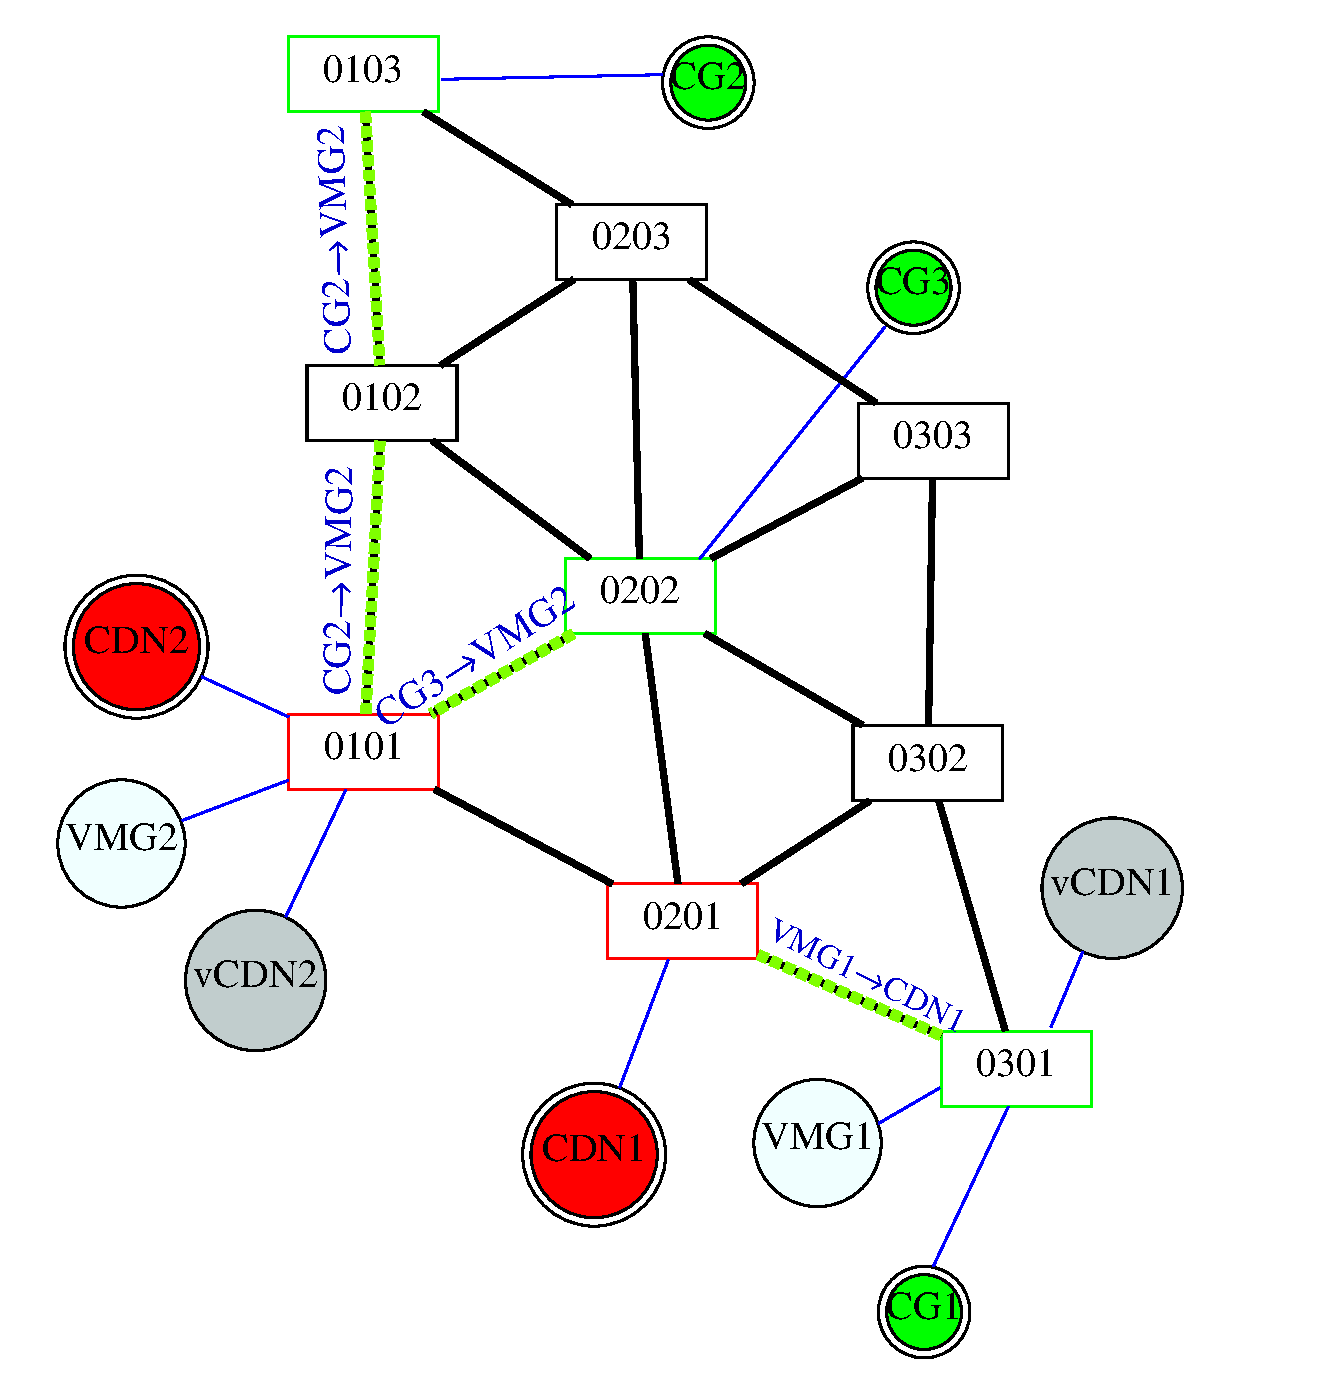
\includegraphics[width=0.90\textwidth]{4x4-2.pdf}}
   \end{center}
  \vspace{0.5em}
  
  
   
   
   

   
 }

 
   \headerbox{Références}{name=ref,column=1,span=2,row=0,below=results}{
   
   [1] Herbaut, N., D. Négru, D. Magoni, and P. A. Frangoudis, "Deploying a Content Delivery Service Function Chain on an SDN-NFV Operator Infrastructure", 2016 International Conference on Telecommunications and Multimedia (TEMU) , Heraklion, IEEE, 07/2016, In Press.
   
   
   [2] Herbaut, N., G. Xilouris, and D. Negru, "The Surrogate vNF approach for Content Distribution", COMSOC Multimedia Communications Technical Committee E-Letter,, vol. 10, pp. 4–6, 2015.
   
   [3] D5.31 - Network Functions Implementation and Testing - T-NOVA WP5 Deliverable http://www.t-nova.eu/results/

    

    
   
    
  
  
  \vspace{1em}
  
 }
   \headerbox{Thanks to}{name=sampleembedding,column=1,span=2,row=0,below=ref}{
 
 
 
\includegraphics[width=0.28\textwidth]{logo_university_of_bordeaux.pdf}   
 
\includegraphics[width=0.10\textwidth]{labri.png}
 
\includegraphics[width=0.40\textwidth]{t-nova.jpg}
 
\includegraphics[width=0.33\textwidth]{vio.jpg}
 
\includegraphics[width=0.25\textwidth]{systematic.png}
 
\includegraphics[width=0.20\textwidth]{temu.png}
 
 
 \vspace{0.5em}
  
 }
 




\end{poster}

\end{document}
